\documentclass[12pt]{article}
    %\usepackage{fullpage}
    \usepackage{epic}
    \usepackage{eepic}
    \usepackage{paralist}
    \usepackage{graphicx}
    \usepackage{enumitem}
    \usepackage{amsmath,amssymb,latexsym,listings}
    \usepackage{algorithm,algorithmic}
    
    \usepackage{tikz}
    \usepackage{xcolor,colortbl}
    \usepackage{wrapfig}
    
    
    %%%%%%%%%%%%%%%%%%%%%%%%%%%%%%%%%%%%%%%%%%%%%%%%%%%%%%%%%%%%%%%%
    % This is FULLPAGE.STY by H.Partl, Version 2 as of 15 Dec 1988.
    % Document Style Option to fill the paper just like Plain TeX.
    
    \typeout{Style Option FULLPAGE Version 2 as of 15 Dec 1988}
    
    \topmargin 0pt
    \advance \topmargin by -\headheight
    \advance \topmargin by -\headsep
    
    \textheight 8.9in
    
    \oddsidemargin 0pt
    \evensidemargin \oddsidemargin
    \marginparwidth 0.5in
    
    \textwidth 6.5in
    %%%%%%%%%%%%%%%%%%%%%%%%%%%%%%%%%%%%%%%%%%%%%%%%%%%%%%%%%%%%%%%%
    
    \pagestyle{empty}
    \setlength{\oddsidemargin}{0in}
    \setlength{\topmargin}{-0.8in}
    \setlength{\textwidth}{6.8in}
    \setlength{\textheight}{9.5in}
    
    
    \def\ind{\hspace*{0.3in}}
    \def\gap{0.1in}
    \def\bigap{0.25in}
    \newcommand{\Xomit}[1]{}
    
    \DeclareMathOperator*{\argmin}{arg\,min}
    \DeclareMathOperator*{\argmax}{arg\,max}
    
    \begin{document}
    \setlength{\parindent}{5ex}
    \addtolength{\parskip}{0.1cm}
    \setlength{\fboxrule}{.5mm}\setlength{\fboxsep}{1.2mm}
    \newlength{\boxlength}\setlength{\boxlength}{\textwidth}
    \addtolength{\boxlength}{-4mm}
    \begin{center}\framebox{\parbox{\boxlength}{{\bf
    CS 4775 \hfill Final Project Report}\\
    Title: \textbf{Re-implementing Coal-HMM} \hfill Dilip Thiagarajan
    }}
    \end{center}
    \section{Introduction}
    Comparative analysis of sequence alignments related by speciation has commonly been understood
    using phylogenetic trees, which quantifies the similarity of physical and genetic
    characteristics. However, one thing that is hard to account for is the possibility of having different evolutionary histories for different parts of the alignment. In this study, we re-implement a simpler form of the the methods outlined in the coalescent Hidden Markov Model paper towards identifying different evolutionary histories for different alignment columns.
    \subsection{Related Work}
    The paper outlining the coalescent Hidden Markov Model, written by Hobolth et. al ([2]), is a more specific form of the general phylogenetic Hidden Markov Model, as delineated by Siepel et.al. ([1]), which considers both changes in space (along the genome), as well as changes in time (along the edges of the tree). To do so, it computes the likelihood of a sequence alignment $X$, given a tree model $T$, using Felsenstein's algorithm. This constitutes the emission probability aspect of the Markov model. Moreover, to model DNA substitution, Siepel et. al defines a general rate matrix parameter $Q$, and in our work, we choose to use the Jukes-Cantor model to calculate this matrix $Q$. In their study, Siepel et. al work towards estimating the likelihood for partitions of the alignment undergoing different evolutionary processes.

    Instead of framing the problem from the perspective of evolutionary processes, Hobolth et. al look to estimate the likelihood of different possible evolutionary histories, by introducing new free parameters and a methodology to estimate population genetic quantities, such as speciation times and ancestral population sizes. Specifically, they introduce parameters defining the branch lengths of the possible phylogenetic trees, and state the algorithm they use to estimate those parameters along with parameters of the transition matrix in their HMM model. Given the time constraint on this project, we assume the branch lengths are fixed to the values they have reported, and study the results of this HMM model (henceforth denoted as coal-HMM) for other target regions in multiple alignments publicly available.
    \subsection{Outline}
    In the following section, we outline the exact methodology in generally analyzing a multiple alignment containing the four genomes analyzed in Hobolth's paper (human, chimp, gorilla, orangutan), as well as all simplifying assumptions that were made. Then, we describe the results of the training procedure, and consequently apply those results to report what genealogy is most likely for each alignment column in various targets. Finally, we discuss the problems of the approach used.
    \section{Methods}
    \subsection{Modeling Assumptions}
    In general, a hidden Markov model is used to model the probability of a sequence of observations, assuming that each observation is emitted from some distribution corresponding to a a hidden state selected from another distribution. Specifically, if we let $x_i, i \in [1,n]$ be the sequence of observations, and if we let $z_i, i \in [1,n]$ be the sequence of associated hidden states for each observation, then the hidden Markov model makes the following assumption (where $\textbf{x}, \textbf{z}$ are the sequence of observations and sequence of hidden states, respectively):
    $$P(\textbf{x}, \textbf{z}) = P(x_1 | z_1)P(z_1) \prod_{i=2}^{n} P(x_i | z_i) P(z_i | z_{i-1})$$
    Explicitly, we make the bigram modeling assumption on the hidden states, i.e. that each hidden state is only dependent on the previous state (save for the first, which depends on some initialization probability distribution), and we assume that each emission is only dependent on the hidden state at that point of time.
    \\ \\
    To compute the probability of just the observations, i.e. $P(\textbf{x})$, we can just marginalize over $\textbf{z}$. Furthermore, by using the forward-backward algorithm, as outlined in class, we can compute the posterior probability of each state $P(z_i = k | \textbf{x})$. Thus, the only thing that needs further specification at this point is the probability of an emission, i.e. $P(x_i | z_i)$ for any $i$, as well as the probability $P(z_i | z_{i-1})$.
    \subsection{Transition and Emission Probability Model}
    As outlined in Hobolth et. al, we use the following matrix $T$ to model transitions between the four states $HC_1, HC_2, HG, CG$:
    $$T = \begin{bmatrix} 1 - 3s & s & s & s \\ u & 1 - (u+2v) & v & v \\ u & v & 1 - (u+2v) & v \\ u & v & v & 1 - (u+2v) \end{bmatrix}$$
    where each entry $t_{ij}$ corresponds to the probability $P(z_j | z_i)$, assuming the ordering above for the four states.

    As a simplification on their study, we compute the likelihood of an alignment column under the Jukes-Cantor model, which models mutations as a Poisson process. Specifically, we model $P(b|a, t)$, the probability of a base $b$ at time $t$ starting from base $a$, as:
    \[ \begin{cases} 
            \frac{1}{4}(1 + 3e^{-\frac{4t}{3}}) & b = a \\
            \frac{1}{4}(1 - e^{-\frac{4t}{3}}) & b \ne a \\
        \end{cases}
    \]
    and with this, we can compute the probability of an alignment column given the phylogenetic tree using Felsenstein's algorithm, which computes the likelihood efficiently using a dynamic approach. The times $t$ are described by the branch lengths of each genealogy, which are described below. The 4 probabilities for each alignment column are normalized so that the 4 probabilities constitute a true probability distribution.
    \subsection{Phylogenetic States}
    Hobolth et. al outline 4 possible states in analyzing the alignment between the human, chimp, gorilla, and orangutan genomes. They are:
    \begin{enumerate}
        \item $HC_1$, which has the human and chimp coalesce first. The postorder traversal will have the leaves traversed in the following order: human, chimp, gorilla, orangutan.
        \item $HC_2$, which has the human and chimp coalesce first again, but at a later time. The postorder traversal will have the leaves traversed in the following order: human, chimp, gorilla, orangutan.
        \item $HG$, which has the human and gorilla coalesce first. The postorder traversal will have the leaves traversed in the following order: human, gorilla, chimp, orangutan.
        \item $CG$, which has the chimp and gorilla coalesce first. The postorder traversal will have the leaves traversed in the following order: chimp, gorilla, human, orangutan.
    \end{enumerate}
    Each of these phylogenies has the same overall structure, which is shown below. For the latter 3, we use the lengths that have primes associated with them, which represent $\widetilde{a}, \widetilde{b}, \widetilde{c}, \widetilde{x}$. Note that $x$ and $\widetilde{x}$ are numbers we've introduced (i.e. not included in Hobolth's study) such that
    $$a + b + x = c - x$$
    $$\widetilde{a} + \widetilde{b} + \widetilde{x} = \widetilde{c} - \widetilde{x}$$
    which models the assumption that the distance to the root is the same for all leaves. In practice, this is a hyperparameter we would tune to maximize the likelihood of the probability of the alignment columns, but this assumption allows us to have a precise definition for $x$, while maintaining all the constraints imposed by Hobolth on this model.

    Also note that the ordering of the leaves (from left to right) is different for each hidden state, and thus introduces the key differences of each hidden state, allowing us to differentiate between the probability of each phylogeny when considering an alignment column.
    \begin{center}
    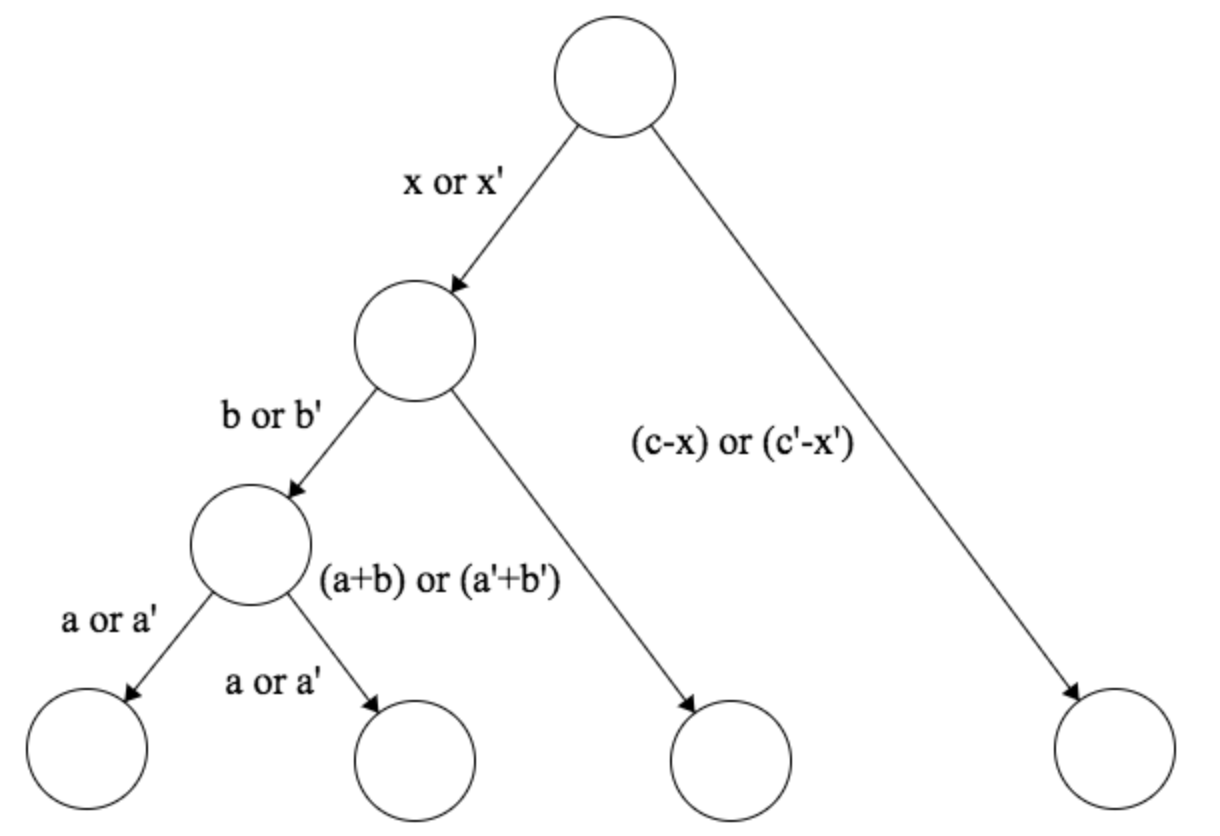
\includegraphics[scale=0.5]{phyl}
    \end{center}
    \subsection{Hidden Markov Model Analysis}
    With that, we now have the means for computing the probability of the sequence of observations (i.e. the alignment columns) using the Forward-Backward algorithm under the above assumptions. However, in order to model that probability the most accurately (by maximizing it), we must tune the parameters of our model.
    \subsubsection{Obtaining the Posterior}
    Using the Forward-Backward algorithm, we can obtain the posterior of a hidden state $k$ at a given time $i$. Specifically, let $f(i, k)$ and $b(i, k)$ be the functions describing the forward and backward algorithm outputs for a time $i$ and a hidden state $k$. Then, we have:
    $$P(z_i = k | \textbf{x}) = \frac{P(\textbf{x}, z_i = k)}{P(\textbf{x})} = \frac{f(i, k)b(i, k)}{P(\textbf{x})}$$
    Thus, we can obtain the posterior for any hidden state at any given time, and normalize to obtain the distribution of the posterior over each hidden state any given time. This will allow us to examine the maximum a posteriori estimate of the genealogy for each alignment column using this model. However, we have to maximize the likelihood $P(\textbf{x})$ before doing so, so we use the EM algorithm, as described below.
    \subsubsection{EM}
    For this study, we choose to fix the branch length values to the values reported in Hobolth's study, and only train the parameters of the transition probabilities - $s, u, v$. To do this, we utilize the Baum-Welch algorithm, which is a form of expectation-maximization that guarantees values of $s, u, v$ that are a local minima of the negative of the likelihood function described by the hidden Markov model. Given a sequence of $n$ observations and $n$ hidden states $(\textbf{x}, \textbf{z})$, and the corresponding matrix of expected transition counts $A$, where $A_{j,k}$ describes the expected number of times $z_{i-1} = j$ and $z_{i} = k$, $i \in [2,n]$, we can utilize the structure of the transition probability matrix $T$ to derive the steps for the EM algorithm. Specifically, given $A$, we have:
    $$s = \frac{\sum_{z \in \{HC_2, HG, CG\}} A_{HC_1, z}}{\sum_{z \in \{HC_1, HC_2, HG, CG\}} A_{HC_1, z}}$$
    $$u = \frac{\sum_{z \in \{HC_2, HG, CG\}} A_{z, HC_1}}{\sum_{z_1 \in \{HC_2, HG, CG\}} \sum_{z_2 \in \{HC_1, HC_2, HG, CG\}} A_{z_1, z_2}}$$
    $$1 - (u + 2v) = \frac{\sum_{z \in \{HC_2, HG, CG\}} A_{z, z}}{\sum_{z_1 \in \{HC_2, HG, CG\}} \sum_{z_2 \in \{HC_1, HC_2, HG, CG\}} A_{z_1, z_2}}$$
    By Baum-Welch, setting these parameters each iteration must increase the likelihood of the observations under our model. Thus, when we run Baum-Welch for an arbitrary number of iterations, the new probability $P(\textbf{x}, \textbf{z}; s, u, v)$ must be higher.
    \section{Training}
    Given the volatility of the Baum-Welch algorithm to overfitting to local maxima, and the opacity of the likelihood function we are trying to optimize, a lot of care must be taken to not overfit. In this context, that would mean a posterior distribution over each alignment column that does not conform to the majority results consistently after each run. To avoid this, we implement a pseudo-validation scheme, where we keep track of all unique posterior (maximum likelihood hidden state for each alignment column based on the posterior, for all alignment columns) and their associated likelihoods from the Forward-Backward algorithm for 10 random initializations of $s, u, v$, and examine this distribution to make sure the variance of the posterior likelihoods is reasonably small. We also cut off the EM algorithm at a fixed number of iterations (usually between 100-500) to ensure that it's not overfitting.
    \section{Results}
        For the results displayed, training was done for at most 100 iterations.
        \subsection{Data}
        We obtained 20-way alignments of assemblies to the human genome from the UCSC Genome Browser, for two target regions: chromosome Y (chrY), and the mitochondrial DNA (chrM), which was used primarily for development purposes. We remove all information from the file except for the sequence data for any alignment column that includes human, chimp, gorilla, and orangutan sequences. These were arbitrary selections, with the only constraint being alignments of a reasonable size, given the time constraint.

        The link to the relevant page is given in the appendix.
        \subsection{Posterior Estimates}
        For each target, we first find the estimate of the posterior log-probability associated with the most probable phylogenetic tree for each alignment column combined. These results are displayed below ($\mu$ and $\sigma$ indicate mean and deviation across the 10 trials).
        \begin{center}
        \begin{tabular}{ |c|c|c| } \hline
        Target & Alignment Columns & Posterior Log-Probabilities $\mu \pm \sigma$ \\ \hline 
        chr21 & 251302 & -348277.0457 $\pm$ N/A \\ \hline
        chr22 & 268275 & --371872.6541 $\pm$ N/A \\ \hline
        chrM & 178 & -102.2279 $\pm$ 89.2130 \\ \hline
        chrY & 6122 & -6733.5669 $\pm$ 1884.0024 \\ \hline
        \end{tabular}
        \end{center}
        The deviations for chromosomes 21 and 22 weren't computed due to time constraints. We assume the likelihood function is approximately convex accordingly, and only run 1 trial.
        \subsection{Parameter Estimates}
        For each target, we report the values at the end of training for $s, u, v$. These results are displayed below ($\mu$ and $\sigma$ indicate mean and deviation across the 10 trials).
        \begin{center}
        \begin{tabular}{ |c|c|c|c| } \hline
        Target & $s$ $\mu \pm \sigma$ & $u$ $\mu \pm \sigma$ & $v$ $\mu \pm \sigma$ \\ \hline
        chr21 & 0.1197 $\pm$ N/A & 0.3195 $\pm$ N/A & 0.1639 $\pm$ N/A \\ \hline
        chr22 & 0.1803 $\pm$ N/A & 0.2547 $\pm$ N/A & 0.0411 $\pm$ N/A \\ \hline
        chrM & 0.0876 $\pm$ 0.0738 & 0.3210 $\pm$ 0.1508 & 0.1234 $\pm$ 0.0914 \\ \hline
        chrY & 0.2054 $\pm$ 0.1125 & 0.1449 $\pm$ 0.0697 & 0.1699 $\pm$ 0.1007 \\ \hline
        \end{tabular}
        \end{center}
        The deviations for chromosomes 21 and 22 weren't computed due to time constraints. We assume the likelihood function is approximately convex accordingly, and only run 1 trial.
        
        With these parameter estimates, we can compute the posterior distribution for each alignment column for all phylogenetic trees by using the mean values of $s, u, v$ as the MLE values.
        \subsection{Posterior Distributions}
        \subsection{Chromosome 21}
        Here are the posteriors for all relevant alignment columns in chromosome 21.
        {\centering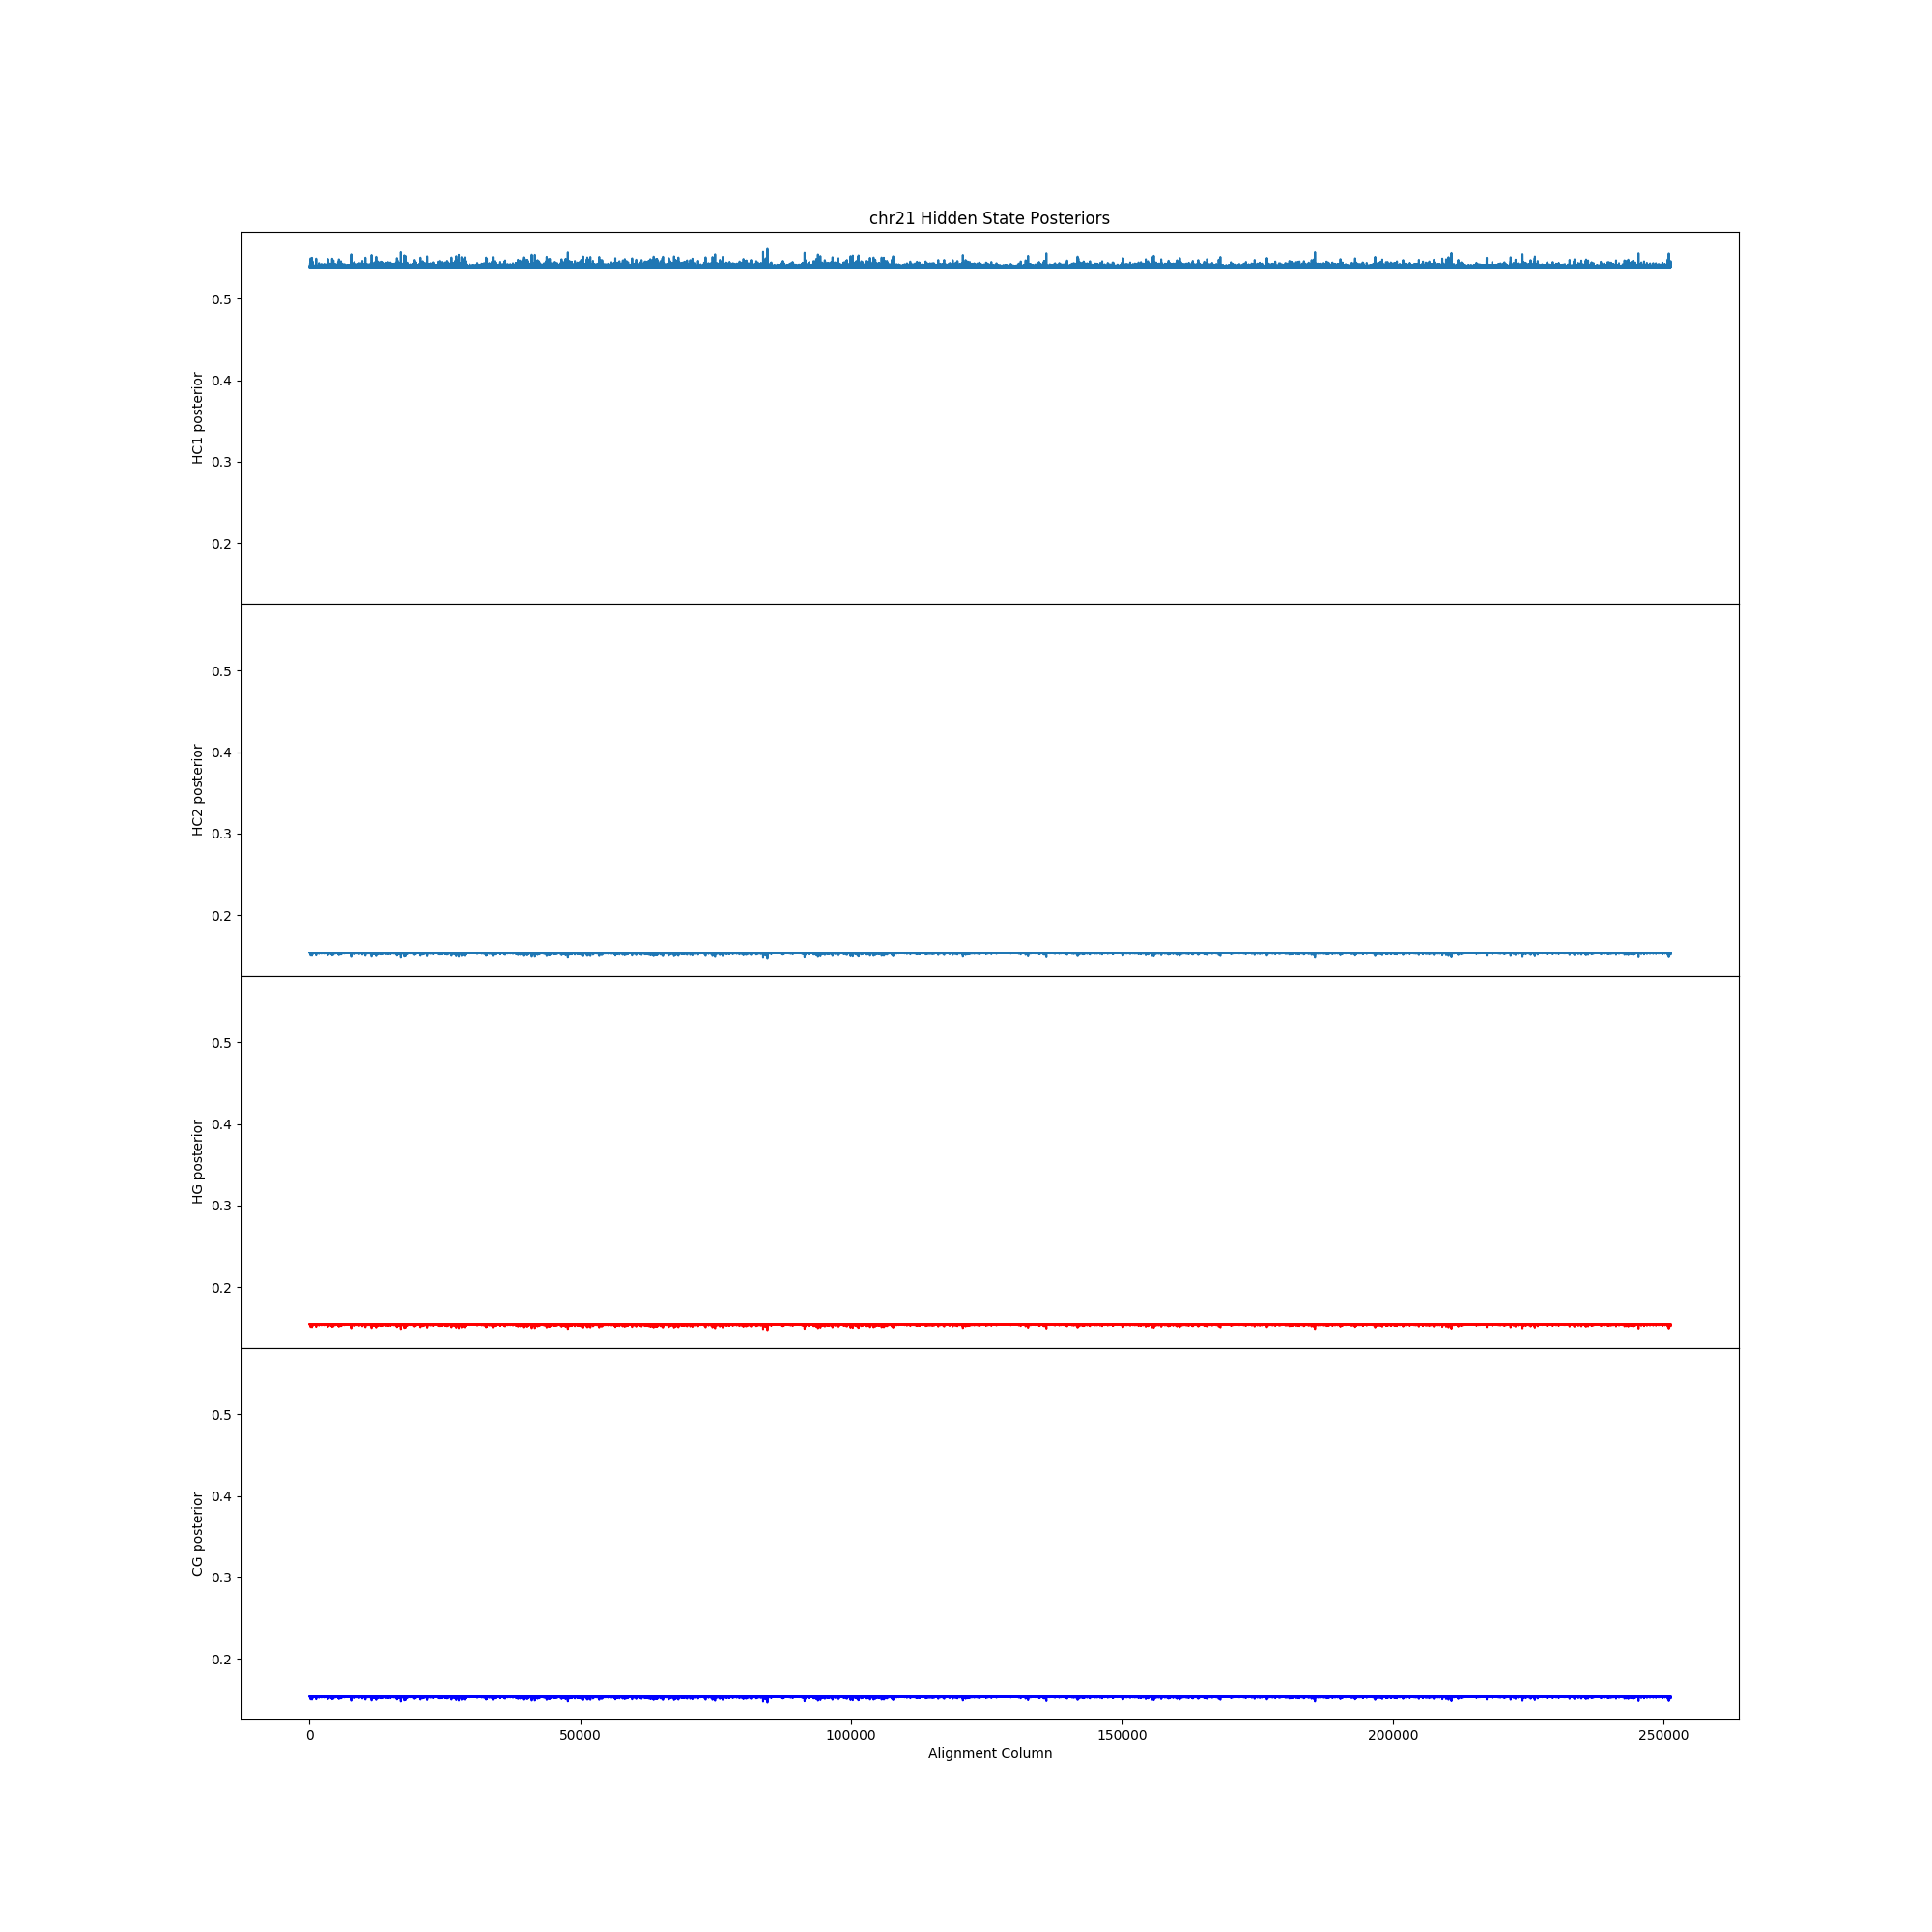
\includegraphics[width=1.\textwidth]{train/chr21_posteriors}\par}
        We see that $HC_1$ is the preferred state over all alignment columns. Full-size images can be found at the repository linked in the appendix, under the train directory.
        \subsection{Chromosome 22}
        Here are the posteriors for all relevant alignment columns in chromosome 22.
        {\centering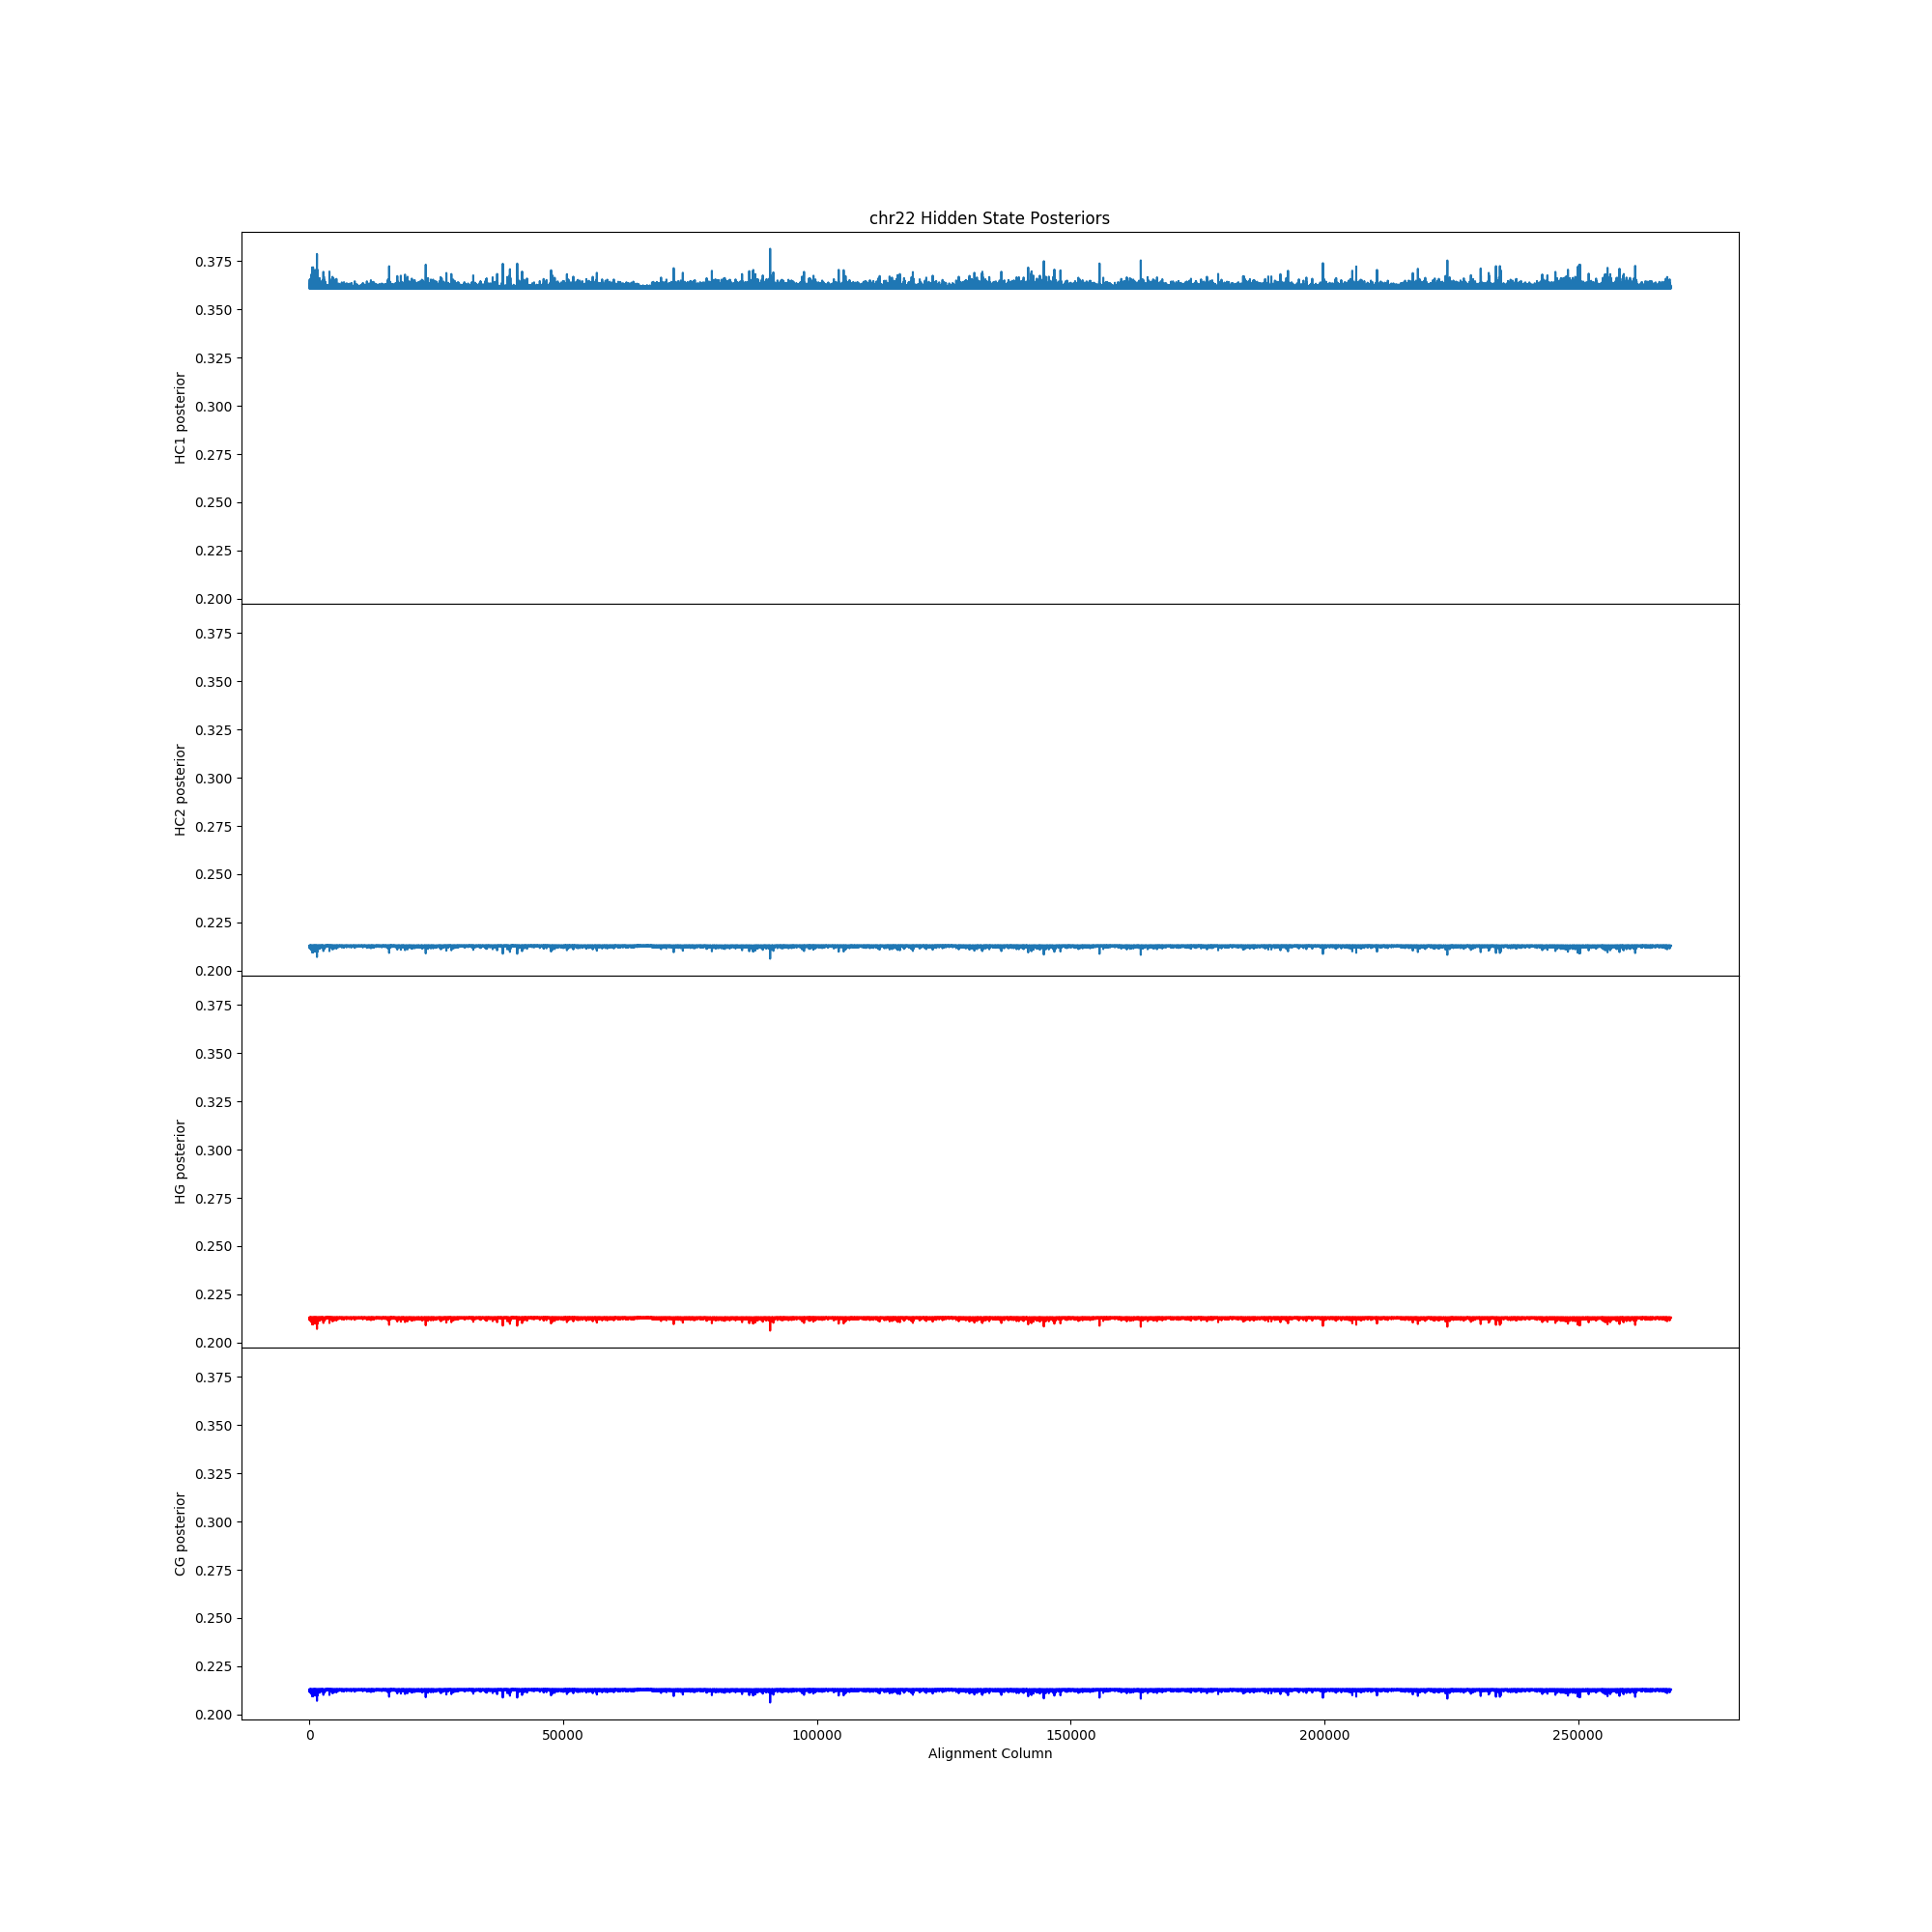
\includegraphics[width=1.\textwidth]{train/chr22_posteriors}\par}
        We see that $HC_1$ is the preferred state over all alignment columns. Full-size images can be found at the repository linked in the appendix, under the train directory.
        \subsubsection{Chromosome M}
        Here are the posteriors for all relevant alignment columns in chromosome M.
        {\centering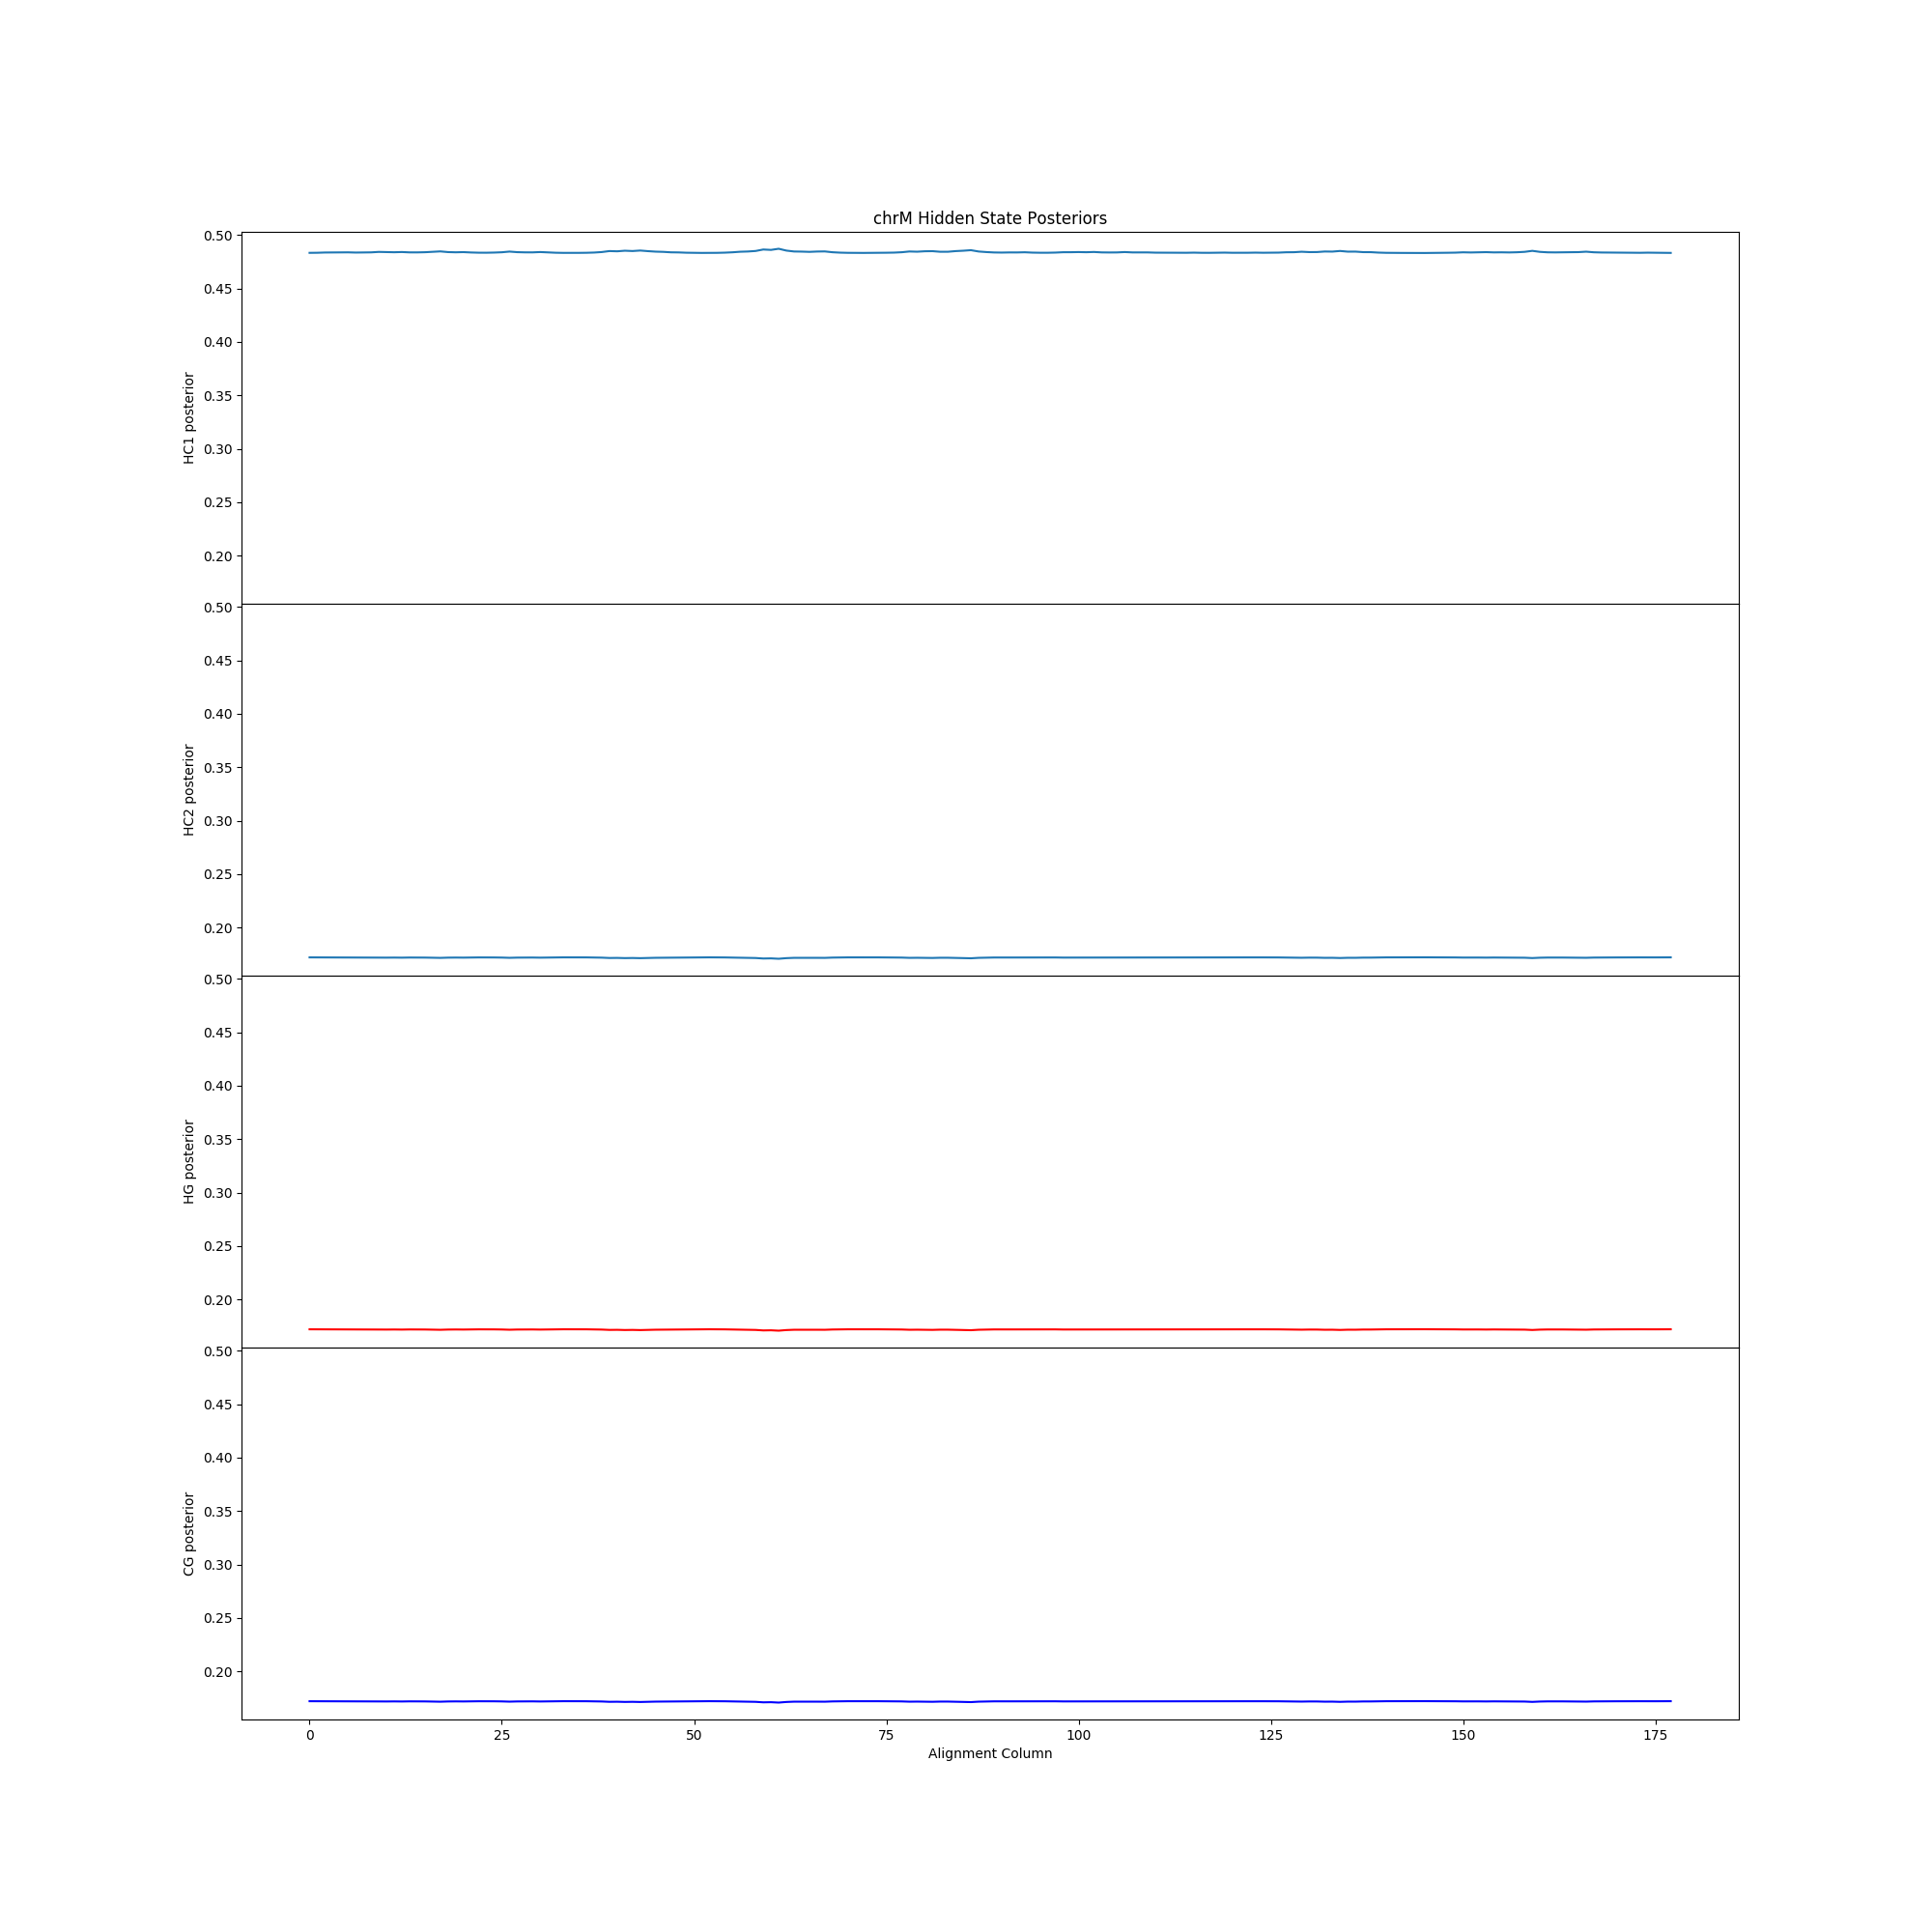
\includegraphics[width=1.\textwidth]{train/chrM_posteriors}\par}
        We see that $HC_1$ is the preferred state over all alignment columns. Full-size images can be found at the repository linked in the appendix, under the train directory.
        \subsubsection{Chromosome Y}
        Here are the posteriors for all relevant alignment columns in chromosome Y.
        {\centering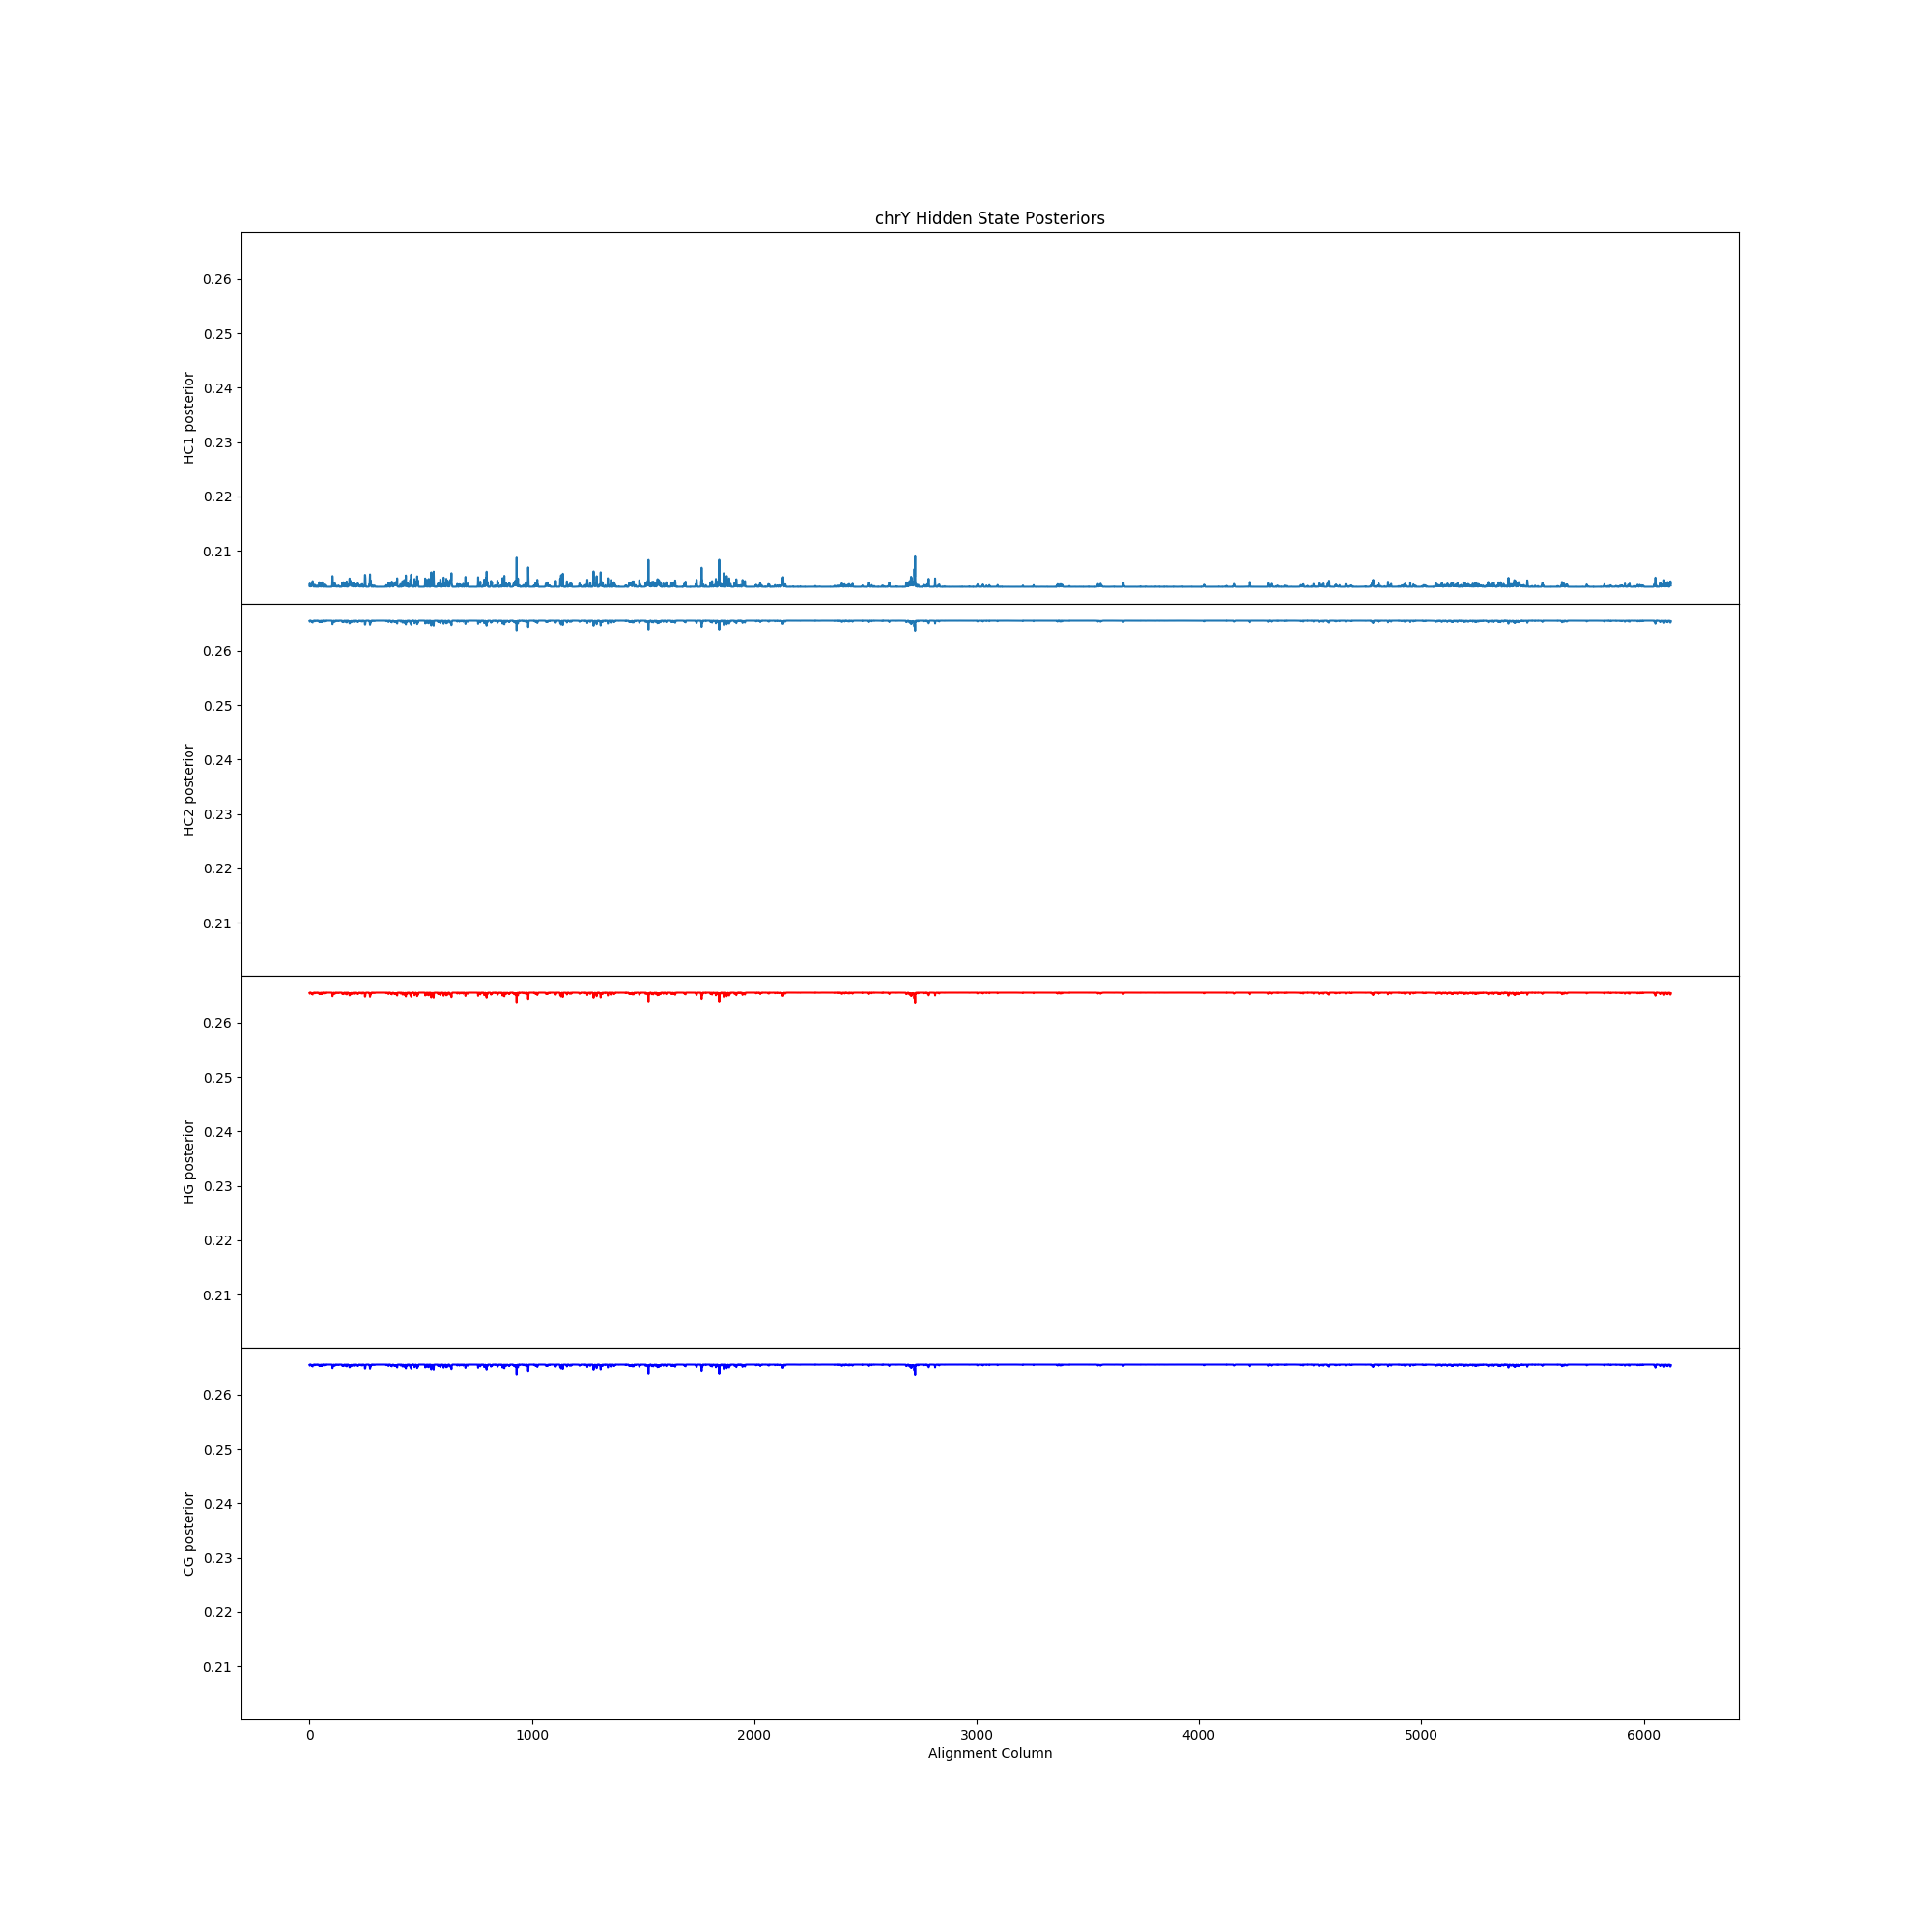
\includegraphics[width=1\textwidth]{train/chrY_posteriors}\par}
        Here, we see that one of $HC_2, HG, CG$ is the preferred state over all alignment columns. Full-size images can be found at the repository linked in the appendix, under the train directory.
    \section{Discussion}
    One thing that's immediately noticeable is the scale of the changes during training in log-likelihood is very small, i.e. on the order $10^{-3}$ or smaller (this can be confirmed by examining the log-likelihood graphs generated by the training procedure). It's possible that the reason that this happens is due to how we fix the branch lengths to the maximum-likelihood estimates as reported in Hobolth's study. Accordingly, the full likelihood function based on all free parameters might have a second derivative that is very low in magnitude around these values for the branch lengths, which would cause the EM algorithm to take a long time, as the function would be very wide and flat around the local maximum, and as a result would require several steps to reach the actual maxima. This posed a major problem, as a significant number of initializations would begin with a log-likelihood close in value to the local maximum achieved for that training trial, and the incremental changes would not make much of a difference in the likelihood or in the posterior distribution. This can be furthermore be seen by the scale of the deviation in both the posterior computations and the parameter estimates being quite large compared to the mean estimate of each. However, this seems to go down as more alignment columns are considered within an individual target, so it's possible that a larger-scale analysis would alleviate this problem.

    Another difference seemed to be in the various values of $s, u, v$ that were found during our study when compared to the values reported by Hobolth et. al. Specifically, we notice that they report very small values of $s, u, v$, with $s, u$ on average being around 0.005 and $v$ being around 0.01 on average, while our study shows $s$ being around 0.15, $u$ being around 0.25, and $v$ being around 0.12. The most likely reason for this is due to how the alignments were obtained, with their alignments being taken from an alignment solely down on humans, chimps, gorillas, and orangutans, while our alignments were taken from a 20-way alignment, so the columns actually correspond more closely to an alignment that would be significant for 20 rather than just the 4.

    Finally, what was most particularly interesting was the lack of significant fluctuation in the posterior of any of the 4 states over a given target chromosome. In Hobolth's study, they find fluctuation in the posterior over the alignment columns. Even though it's not particularly accurate to compare the value of the posteriors, it's interesting that our study found almost no fluctuation in these posterior distributions until the number of alignment columns came to the order of 1000. This indicated that the posterior distribution was heavily governed by the emission probability as opposed to the transition probability.

    Nevertheless, one similarity we do find in our results that is also mentioned in the paper is the strong preference of the Markov model towards $HC_1$ over every other state the majority of time. Hobolth also finds this, mentioning that "the alternative states HC2, HG, and CG are less strongly supported and typically cover very short segments." This is supported by our figures of the posterior distribution for each alignment column - in the mitochondrial DNA, we find that it is completely dominated by $HC_1$, while the DNA in the $Y$ chromosome is dominated by the other 3, with equal probablity. This seems to be the case because in the $Y$ chromosome, most of the alignments have the chimp, gorilla, and orangutan having the same bases, but differ from the human base.
    
    \section{Conclusions}
    In this study, we reimplement a simplification of the coal-HMM model presented by Hobolth et. al, and examine the results for target regions obtained from the UCSC Genome Browser. We find that while some of the numerical results vary due possibly to how the simplification was rationalized and to the difference in base sequences of the various target regions, the theme of the most common state occurring quite frequently as the majority is recurrent in our study as well.
    \section{References}
    \begin{enumerate}
    \item Siepel A, Haussler D (2004) Combining phylogenetic and hidden Markov models in biosequence
            analysis. J Comput Biol 11: 413428.A. SiepelD. Haussler2004Combining phylogenetic
            and hidden Markov models in biosequence analysis.J Comput Biol11413428
    \item Hobolth A, Christensen OF, Mailund T, Schierup MH (2007) Genomic relationships and
            speciation times of human, chimpanzee, and gorilla inferred from a coalescent hidden
            markov model. PLoS Genet 3: e7.
    \end{enumerate}
    \section{Appendix}
    % TODO: Link to code online should be here.
    All data was obtained from http://hgdownload.soe.ucsc.edu/goldenPath/hg38/multiz20way/.
    \end{document}
    